\documentclass[10pt, a4paper]{beamer}

% ---------- Packages ----------
\usepackage[utf8]{inputenc}
\usepackage[english]{babel}
\usepackage{amsmath}
\usepackage{amsfonts}
\usepackage{amssymb}
\usepackage{colortbl}
\usepackage{tikz}
\usetikzlibrary{mindmap,calc,shapes,arrows,shapes.geometric,decorations.markings,patterns,decorations.pathmorphing,positioning}

% ---------- Template setup ----------
\mode<presentation>
\setbeamertemplate{headline}%
{%
	\begin{beamercolorbox}[rounded=true, center, wd=\paperwidth]{bgcolor}%
		\begin{columns}[T]%
			\begin{column}{9cm}%
				\vspace{2pt}%
				{\color{gray}\tiny Hochschule Emden/Leer} \\%
				{\color{gray}\tiny Abteilung Maschinenbau} \\%
				{\color{gray}\tiny MSR-Labor}%
			\end{column}%
			\begin{column}{2cm}%
				
\includegraphics[scale=0.25]{technik.jpg}%
			\end{column}%
		\end{columns}%
	\end{beamercolorbox}%
	\vspace{10pt}%
}

\setbeamertemplate{navigation symbols}{}
\setbeamertemplate{sidebar right}{}
\setbeamertemplate{sidebar left}{}

\usetheme{default}
\useinnertheme[shadow=true]{rounded}
\usebackgroundtemplate
{%
	\rule{0pt}{\paperheight}%
	\hspace*{\paperwidth}%
	\makebox[0pt][r]{
\includegraphics[width=\paperwidth]{hintergrund2.png}}%
}

\definecolor{HSELhellblau}{RGB}{138,198,203}
\definecolor{HSELblau}{RGB}{0,59,95}
\usecolortheme[named=HSELblau]{structure}

\setbeamertemplate{section}[numbered]
\setbeamertemplate{bibliography item}{\insertbiblabel}

\newcommand{\STANDARD}[2]
{
	\mode<presentation>%
	{%
		\begin{frame}[allowframebreaks]{#1} #2 \end{frame}
	}%
}

% ---------- Metadata ----------
\title{AI-Powered Project Monitoring Tool}
\subtitle{ML-Based Task Allocation, Duration and Delay-Risk Prediction}
\author{%
	Gargi Nilesh Barve\\[1mm]
	{\footnotesize}
	\and
	Rushikesh Suresh Jadhav\\[1mm]
	{\footnotesize}
}
\date{\today}

\setbeamertemplate{footline}{%
	\vspace*{-.1cm}\hspace*{.5cm}
	\scriptsize{\hspace{325pt}\insertframenumber/\inserttotalframenumber}
}

\begin{document}
	
	\setbeamercolor{bgcolor}{fg=black,bg=white}
	
	% ---- 1: Title ----
	\STANDARD{}{\titlepage}
	
	% ---- 2: Table of contents ----
	\section{Introduction}
	\section{Proposed Approach}
	\section{Workflow}
	\section{Evaluation Plan}
	\section{Future Scope and Learnings}
	\section{References}
	\STANDARD{}{\tableofcontents[hideallsubsections]}
	\setbeamercovered{transparent}
	
	% ================= INTRODUCTION =================
	
	% ---- 3 ----
	\STANDARD{The Problem}
	{
		\framesubtitle{Why Project Monitoring Needs to Change}
		\begin{itemize}
			\item Only around 35\% of projects are considered successful; one cause is the low maturity of the tools used to manage them \cite{nenni2025}
			\item Most teams still rely on spreadsheets and manual status updates, so delays are noticed late
			\item Task assignment is usually based on a manager's intuition, not on skills, past performance, or current workload \cite{alfraihat2024}
			\item Predictive features (delay risk, effort forecasting) are rare or locked behind enterprise tools
		\end{itemize}
	}
	
	% ---- 4 ----
	\STANDARD{What Is the Project?}
	{
		\framesubtitle{Project Objective}
		\begin{itemize}
			\item A Jira-style project monitoring tool with \textbf{trained ML models} instead of fixed rules
			\item \textbf{Task allocation:} recommend the best employee for a task based on skills, past performance, workload, and customer category (e.g.\ repeat or high-budget customers)
			\item \textbf{Duration prediction:} estimate how long a task will actually take
			\item \textbf{Delay-risk scoring:} flag tasks likely to miss their deadline
			\item \textbf{Real-time dashboards:} managers see employee performance and project status in one place
		\end{itemize}
	}
	
	% ---- 5 ----
	\STANDARD{Why ML for Project Management?}
	{
		\framesubtitle{State of Research}
		\begin{itemize}
			\item Machine learning is the dominant AI technique in project management research, and forecasting is its most common function \cite{taboada2023}
			\item AI is increasingly applied to project risk management across the whole project lifecycle \cite{nenni2025}
			\item Effort estimation is heavily studied, but resource allocation and activity duration have received far less attention \cite{koszykowski2026}
			\item Fully autonomous scheduling is unrealistic today; automating selected subprocesses is the practical path \cite{koszykowski2026}
		\end{itemize}
	}
	
	% ================= PROPOSED APPROACH =================
	
	% ---- 6 ----
	\STANDARD{System Architecture}
	{
		\framesubtitle{How the Pieces Fit Together}
		\begin{itemize}
			\item \textbf{Data layer:} SQLite database as the single source of truth
			\item \textbf{ML layer:} scikit-learn models trained on historical task data, retrained as new tasks complete
			\item \textbf{Application layer:} multi-page Streamlit app --- Dashboard, Tasks, Employees, Customers, ML Insights
			\item \textbf{Tech stack:} Python, pandas, scikit-learn, SQLite, Streamlit
		\end{itemize}
	}
	
	% ---- 7 ----
	\STANDARD{Database Design}
	{
		\framesubtitle{Core Tables}
		\begin{itemize}
			\item \textbf{Employees:} skills, experience level, current workload, performance history
			\item \textbf{Tasks:} required skills, priority, complexity, estimated hours, deadline, status, assignee
			\item \textbf{Customers:} category (new, repeat, high-budget), linked projects
			\item \textbf{Task history:} actual hours, completed on time or not, quality outcome --- the training data for all ML models
		\end{itemize}
	}
	
	% ---- 8 ----
	\STANDARD{ML Model 1: Task Allocation}
	{
		\framesubtitle{Who Should Do This Task?}
		\begin{itemize}
			\item \textbf{Step 1 --- Skill match:} cosine similarity between the task's required skills and each employee's skill profile filters suitable candidates
			\item \textbf{Step 2 --- Suitability model:} a Random Forest classifier predicts the probability that an employee completes the task on time and with good quality
			\item Features: skill match, experience, past on-time rate, current workload, task priority and complexity, customer category
			\item Output: a \textbf{ranked list} of employees; the manager makes the final choice
			\item Grounded in ML-based work assignment \cite{anvik2006} and Random Forest task allocation \cite{alfraihat2024}
		\end{itemize}
	}
	
	% ---- 9 ----
	\STANDARD{ML Models 2 and 3: Duration and Risk}
	{
		\framesubtitle{How Long Will It Take? Will It Be Late?}
		\begin{itemize}
			\item \textbf{Duration prediction:} Random Forest regressor predicting actual hours from estimated hours, complexity, priority, and the assignee's experience and workload
			\item Tree-based models are among the most used and effective ML techniques for effort and duration estimation \cite{koszykowski2026}
			\item \textbf{Delay-risk scoring:} Random Forest classifier predicting the probability that a task misses its deadline
			\item Risk prediction is one of the main uses of AI in project management \cite{nenni2025, taboada2023}
			\item Delayed tasks are usually the minority class, so class balancing (e.g.\ SMOTE) will be applied \cite{alfraihat2024}
		\end{itemize}
	}
	
	% ================= WORKFLOW =================
	
	% ---- 10 ----
	\begin{frame}{System Workflow}
		\framesubtitle{From Task Entry to Manager Decision}
		\centering
		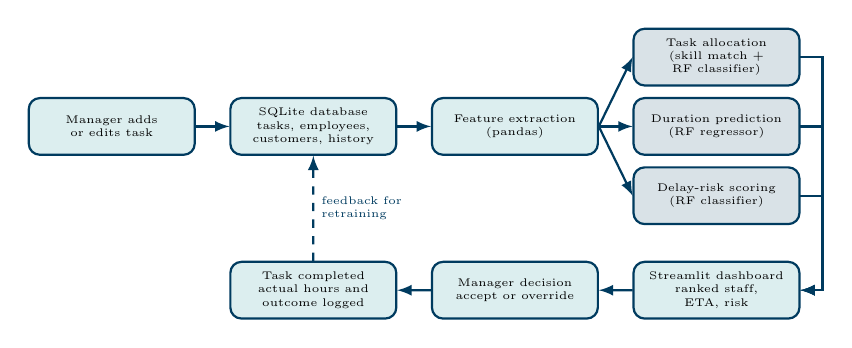
\begin{tikzpicture}[scale=0.8, transform shape,
			box/.style={rectangle, rounded corners, draw=HSELblau, thick,
				fill=HSELhellblau!30, text width=2.4cm, align=center,
				minimum height=0.9cm, font=\tiny},
			ml/.style={box, fill=HSELblau!15},
			arr/.style={-latex, thick, HSELblau}]
			
			% Row 1
			\node[box] (A) at (0,0)   {Manager adds or edits task\\};
			\node[box] (B) at (3.2,0) {SQLite database\\tasks, employees, customers, history};
			\node[box] (C) at (6.4,0) {Feature extraction\\(pandas)};
			
			% ML models
			\node[ml] (M1) at (9.6,1.1)  {Task allocation\\(skill match + RF classifier)};
			\node[ml] (M2) at (9.6,0)    {Duration prediction\\(RF regressor)};
			\node[ml] (M3) at (9.6,-1.1) {Delay-risk scoring\\(RF classifier)};
			
			% Row 2
			\node[box] (D) at (9.6,-2.6) {Streamlit dashboard\\ranked staff, ETA, risk};
			\node[box] (E) at (6.4,-2.6) {Manager decision\\accept or override};
			\node[box] (F) at (3.2,-2.6) {Task completed\\actual hours and outcome logged};
			
			% Arrows
			\draw[arr] (A) -- (B);
			\draw[arr] (B) -- (C);
			\draw[arr] (C.east) -- (M1.west);
			\draw[arr] (C) -- (M2);
			\draw[arr] (C.east) -- (M3.west);
			\draw[arr] (M1.east) -- ++(0.35,0) |- (D.east);
			\draw[arr] (M2.east) -- ++(0.35,0) |- (D.east);
			\draw[arr] (M3.east) -- ++(0.35,0) |- (D.east);
			\draw[arr] (D) -- (E);
			\draw[arr] (E) -- (F);
			\draw[arr, dashed] (F) -- node[right, font=\tiny, text width=1.6cm] {feedback for retraining} (B);
		\end{tikzpicture}
	\end{frame}
	
	% ================= EVALUATION =================
	
	% ---- 11 ----
	\STANDARD{Evaluation Plan}
	{
		\framesubtitle{How We Will Measure the Models}
		\begin{itemize}
			\item \textbf{Data split:} 80/20 train/test split plus k-fold cross-validation \cite{alfraihat2024}
			\item \textbf{Task allocation:} precision of the top-1 and top-3 recommendations \cite{anvik2006}
			\item \textbf{Duration prediction:} mean absolute error (hours) and $R^2$
			\item \textbf{Delay risk:} precision, recall, F1-score, and ROC-AUC --- not accuracy alone, since classes are imbalanced
			\item \textbf{Baseline:} compare each model against the earlier rule-based version of the tool
		\end{itemize}
	}
	
	% ================= FUTURE SCOPE & LEARNINGS =================
	
	% ---- 12 ----
	\STANDARD{Future Scope}
	{
		\framesubtitle{Beyond This Build}
		\begin{itemize}
			\item Train on real Jira, Asana, or GitHub data instead of synthetic data lack of real datasets is a known challenge in this field \cite{koszykowski2026}
			\item Use NLP on task descriptions as additional features, as in text-based assignment \cite{anvik2006, alfraihat2024}
			\item Explainability: show managers \emph{why} a task was flagged or an employee was recommended
			\item Richer resourcing: leave calendars and multi-project contention
			\item Move to a scalable backend (API layer, PostgreSQL) for multi-user use
		\end{itemize}
	}
	
	% ---- 13 ----
	\STANDARD{Learnings So Far}
	{
		\framesubtitle{What This Project Has Taught Us}
		\begin{itemize}
			\item Rule-based scoring is easy to build but cannot learn from past outcomes a trained model can
			\item Data quality and quantity decide model quality; assignment accuracy depends on having enough past tasks per person \cite{anvik2006}
			\item High accuracy can be misleading on imbalanced data, so F1 and AUC matter \cite{alfraihat2024}
			\item ML should support the manager, not replace them: recommend, then let a human decide \cite{anvik2006, koszykowski2026}
		\end{itemize}
	}
	
	% ================= REFERENCES =================
	
	% ---- 14 ----
	\begin{frame}[allowframebreaks]{References}
		\scriptsize
		\begin{thebibliography}{ASA+24}
			
			\bibitem[AHM06]{anvik2006}
			J.~Anvik, L.~Hiew, and G.~C.~Murphy,
			``Who should fix this bug?,''
			in \emph{Proc. 28th Int. Conf. on Software Engineering (ICSE)}, Shanghai, China, 2006, pp.~361--370,
			doi: 10.1145/1134285.1134336.
			
			\bibitem[ASA+24]{alfraihat2024}
			D.~Al-Fraihat, Y.~Sharrab, A.-R.~Al-Ghuwairi, H.~Alzabut, M.~Beshara, and A.~Algarni,
			``Utilizing machine learning algorithms for task allocation in distributed agile software development,''
			\emph{Heliyon}, vol.~10, e39926, 2024,
			doi: 10.1016/j.heliyon.2024.e39926.
			
			\bibitem[KO26]{koszykowski2026}
			M.~Koszykowski and W.~Orzeszko,
			``Machine learning in project schedule creation: A systematic literature review,''
			\emph{Journal of Scheduling}, vol.~29, pp.~21--38, 2026,
			doi: 10.1007/s10951-025-00857-w.
			
			\bibitem[NDDF25]{nenni2025}
			M.~E.~Nenni, F.~De Felice, C.~De Luca, and A.~Forcina,
			``How artificial intelligence will transform project management in the age of digitization: A systematic literature review,''
			\emph{Management Review Quarterly}, vol.~75, pp.~1669--1716, 2025,
			doi: 10.1007/s11301-024-00418-z.
			
			\bibitem[TDTV23]{taboada2023}
			I.~Taboada, A.~Daneshpajouh, N.~Toledo, and T.~de Vass,
			``Artificial intelligence enabled project management: A systematic literature review,''
			\emph{Applied Sciences}, vol.~13, no.~8, p.~5014, 2023,
			doi: 10.3390/app13085014.
			
		\end{thebibliography}
	\end{frame}
	
\end{document}